%!TEX root = ../../tcc.tex

\section{Threads}

\Glspl{thread} são procedimentos que são executados de forma independente do programa
principal, sujeitos ao escalonamento de processos do sistema operacional. Suas
implementações dependem do sistema, porém as linguagens de programação provêm meios de
um programador criar e terminar \glspl*{thread}. Especificamente em sistemas UNIX, uma
implementação é a \emph{POSIX} (\emph{Portable Operating System Interface}),
que é uma família de padrões da IEEE (\emph{Institute of Electrical and Electronics
Engineers}) \cite{site:posixthread}.

Processos contêm várias informações sobre recursos e estados de execução de um programa:

\begin{itemize}
    \item IDs de processo, de grupo de processo, de grupo de usuário e de usuário;
    \item ambiente;
    \item diretório de trabalho;
    \item registradores;
    \item pilha de chamada;
    \item \emph{heap};
    \item descritores de arquivos;
    \item ações de sinal;
    \item bibliotecas compartilhadas;
    \item comunicações inter-processos.
\end{itemize}

\begin{figure}[H]
    \centering
    \fbox{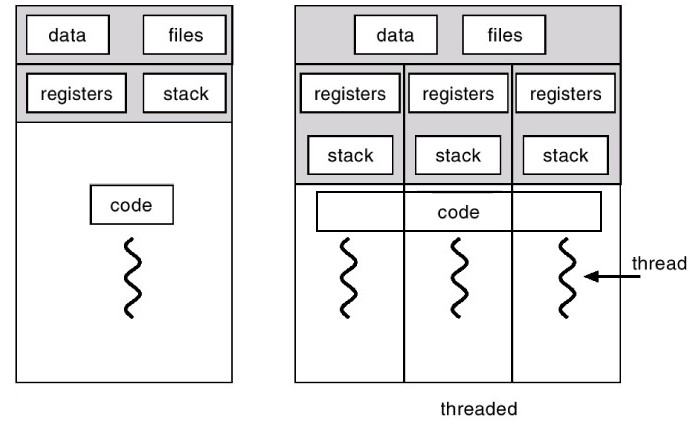
\includegraphics[width=\textwidth]{threads.jpg}}
    \caption{estruturas de processos UNIX, sem e com threads. Fonte:\cite{site:posixthread2}}
    \label{fig:threads}
\end{figure}

Quando uma \gls*{thread} é criada pelo sistema operacional, ela passa a existir dentro
dos recursos do processo. Esses recursos poderão ser usados por ela, inclusive de forma
compartilhada com outras \glspl*{thread}. Na sua criação, alguns desses recursos são
duplicados para uso próprio, o que permite sua execução independentemente do processo
pai, enquanto este existir.

Apesar da praticidade e poder computacional que permite, um problema surge, que é o uso
de memória compartilhada. Assim, \glspl*{thread} precisam ter a leitura e escrita de
dados sincronizada, para que se garanta que esses dados já tenham sido preparados por
uma \gls*{thread} quando outra quiser acessá-los, por exemplo. O estudo dessas
sincronizações e de processamentos independentes entre \glspl*{thread} é o objetivo da
área de Computação Paralela e Concorrente.

O Transmission controla as chamadas de funções a serem executadas em \glspl*{thread},
usando uma estrutura que contém a função passada e seus parâmetros de entrada.

\begin{ccode}
// Estrutura de thread do Transmission
// ./libtransmission/platform.c:80
struct tr_thread {
    void            (* func)(void *);
    void             * arg;
    tr_thread_id       thread;
#ifdef WIN32
    HANDLE             thread_handle;
#endif
};
\end{ccode}

Então, encapsula a chamada de novas \glspl*{thread} com a criação do respectivo objeto.
Assim, consegue executar tarefas mais complexas sem que a execução do programa tenha seu
desempenho prejudicado por travamento. Dois exemplos de uso de criação de
\glspl*{thread} são: para o \gls{bootstrap} da \gls{dht}, e para efetuar requisições a
\glspl{tracker}.

\cfile[label="./libtransmission/platform.c:156"]{./Codes/chap4/021-thread.c}

Outro recurso que o Transmission utiliza são as travas (\emph{locks}), que servem para
controlar o acesso a uma variável durante um programa de várias \glspl*{thread}. Com
isso, garante que a escrita em uma variável não ocorra simultaneamente à uma leitura.

\cfile[label="./libtransmission/platform.c:139"]{./Codes/chap4/022-thread-lock.c}